\documentclass[11pt,letterpaper]{article}
\usepackage[margin=1in]{geometry}
\usepackage{amsmath}
\usepackage{graphicx}
\usepackage{caption}
\usepackage{subcaption}
\usepackage{booktabs}
\usepackage{hyperref}

\begin{document}

\section*{Computational Modeling of Interfacial Stability}

\subsection*{Chemical Stability}

The chemical reaction energies between each cathode material and the five halide
solid electrolytes (SEs) were computed using the \texttt{InterfacialReactivity}
module in \texttt{pymatgen}, with thermodynamic data retrieved from the Materials
Project database. Figure~\ref{fig:chem_fef3} and Figure~\ref{fig:chem_fecl3}
show the chemical reaction energy as a function of the cathode molar fraction
for FeF$_3$ and FeCl$_3$, respectively. The molar fraction $x$ is defined as
$x = n_\mathrm{cathode}/(n_\mathrm{cathode} + n_\mathrm{SE})$, and the
reaction energy is normalized per atom of the reactant mixture. A negative
value indicates thermodynamic instability at that composition.

\begin{figure}[htbp]
  \centering
  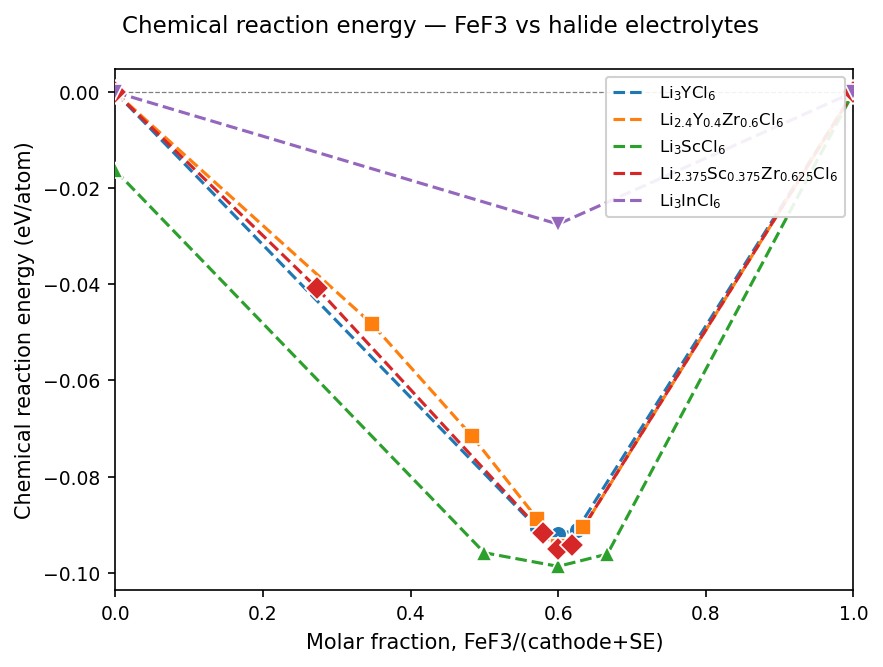
\includegraphics[width=0.5\textwidth]{../chemical_stability_FeF3.png}
  \caption{Chemical reaction energy between FeF$_3$ and five halide solid
           electrolytes as a function of cathode molar fraction. Markers
           indicate kink compositions where the decomposition products change.}
  \label{fig:chem_fef3}
\end{figure}

\begin{figure}[htbp]
  \centering
  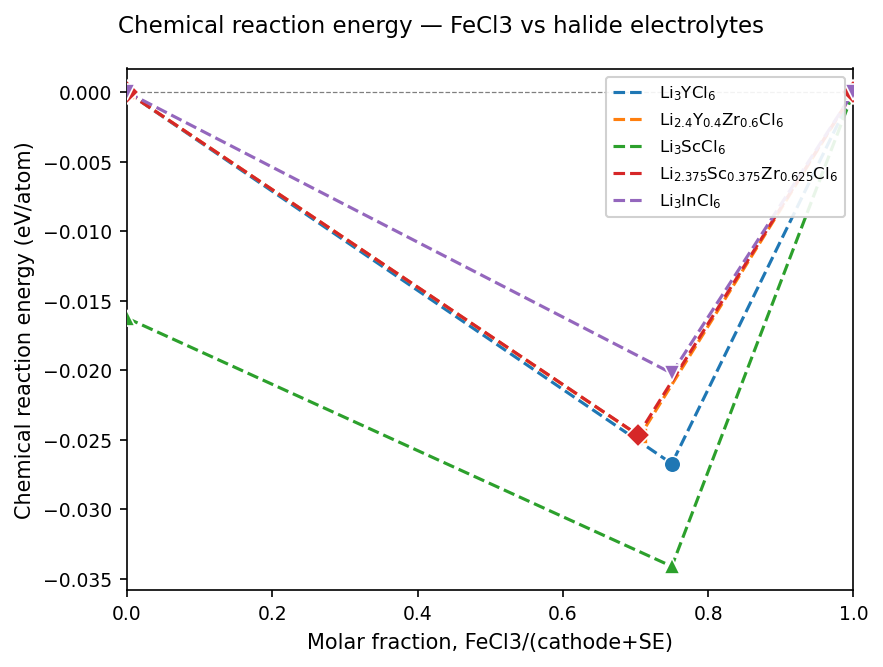
\includegraphics[width=0.5\textwidth]{../chemical_stability_FeCl3.png}
  \caption{Chemical reaction energy between FeCl$_3$ and five halide solid
           electrolytes as a function of cathode molar fraction.}
  \label{fig:chem_fecl3}
\end{figure}

\subsection*{Electrochemical Stability}

The electrochemical stability was evaluated using the grand-potential phase
diagram (GPCD) formalism, in which Li is treated as an open element exchanged
with a reservoir at chemical potential $\mu_\mathrm{Li} = \mu_\mathrm{Li}^\mathrm{ref} - V$,
where $V$ is the electrode voltage versus Li/Li$^+$. The reaction energy was
computed across the voltage window of 1.0--4.2\,V in steps of 0.01\,V, with
curves colored from blue (1.0\,V) to red (4.2\,V) following a coolwarm
colormap. Figures~\ref{fig:echem_fef3} and~\ref{fig:echem_fecl3} show the
resulting voltage-dependent reaction energy profiles for FeF$_3$ and FeCl$_3$,
respectively.

\begin{figure}[htbp]
  \centering
  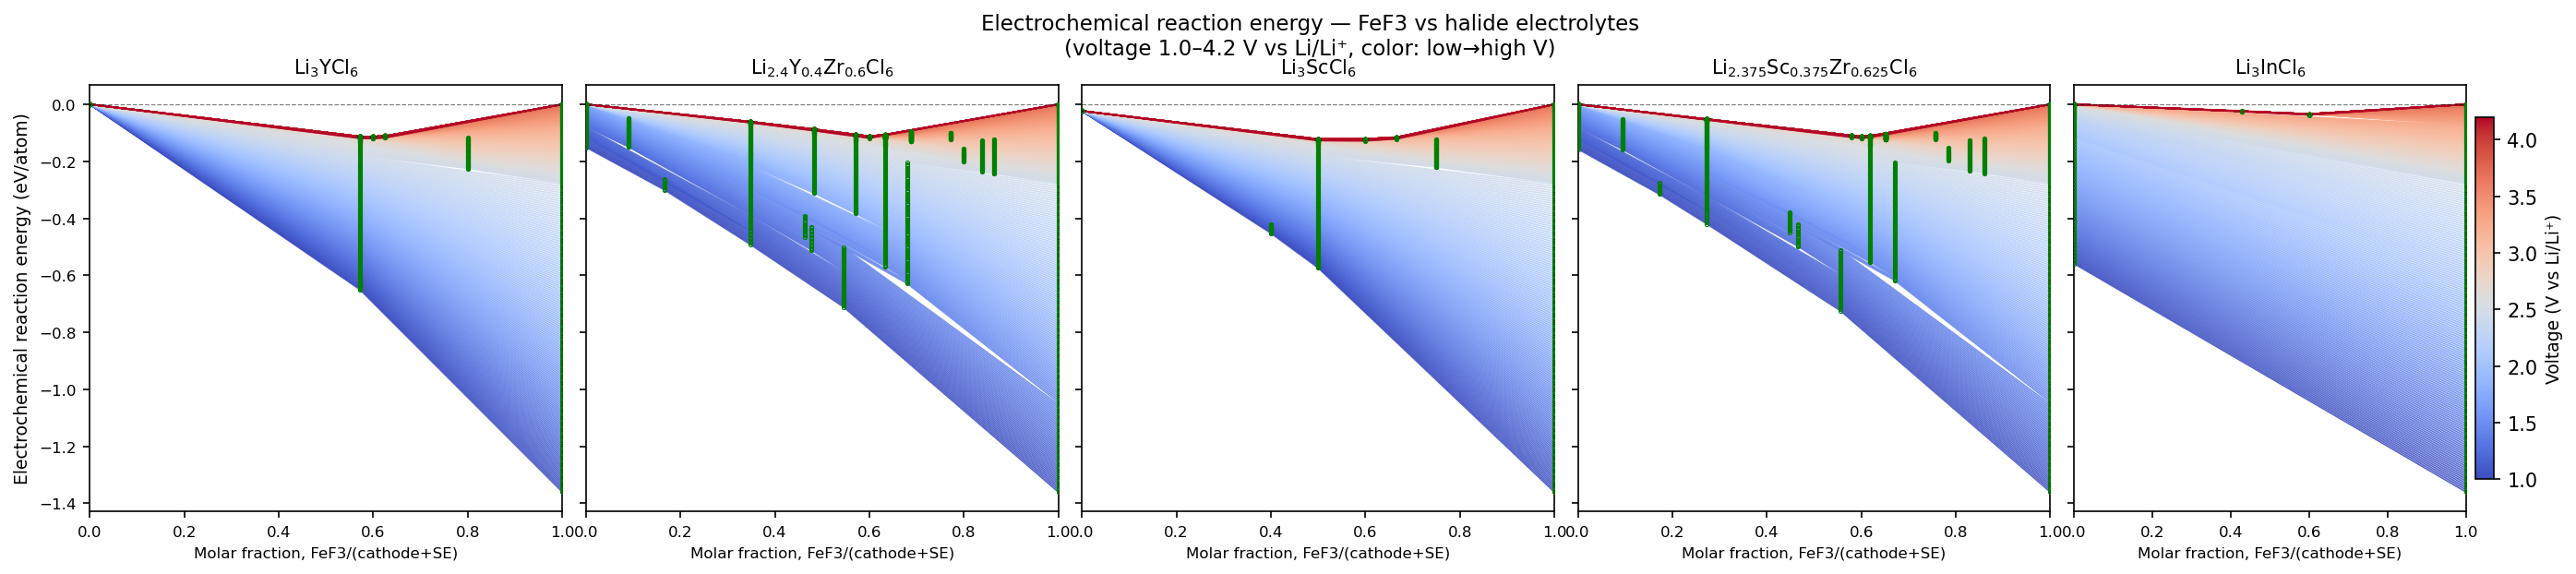
\includegraphics[width=\textwidth]{../electrochemical_stability_FeF3.png}
  \caption{Electrochemical reaction energy between FeF$_3$ and each of the
           five halide solid electrolytes at voltages from 1.0\,V (blue) to
           4.2\,V (red) vs.\ Li/Li$^+$. Green hollow circles mark kink
           positions where the stable decomposition products change.}
  \label{fig:echem_fef3}
\end{figure}

\begin{figure}[htbp]
  \centering
  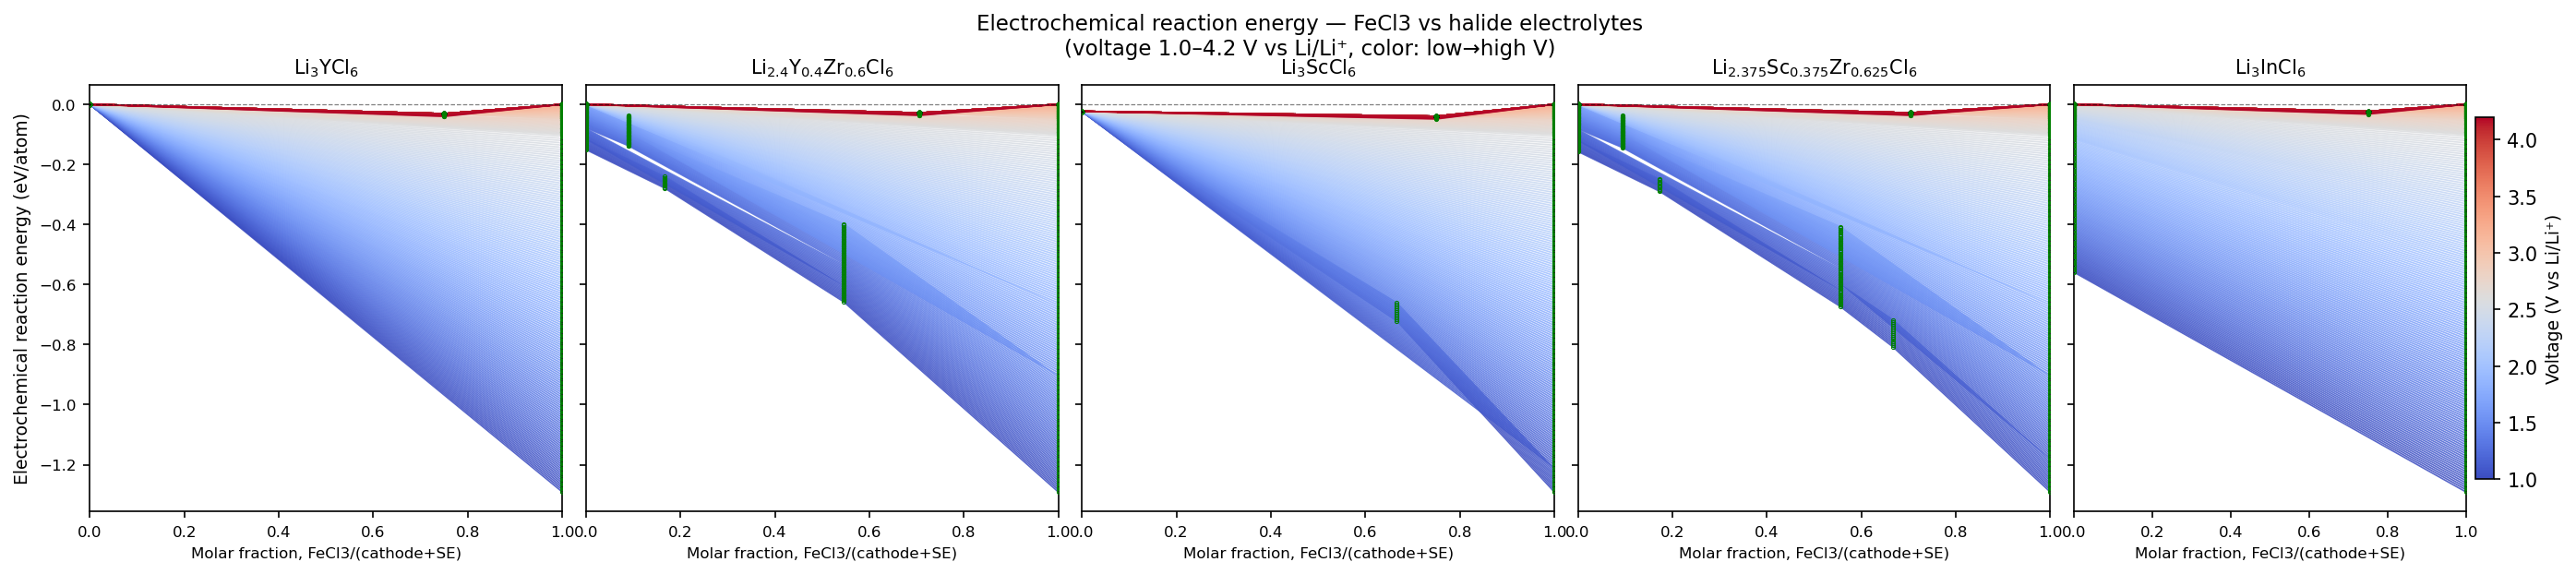
\includegraphics[width=\textwidth]{../electrochemical_stability_FeCl3.png}
  \caption{Electrochemical reaction energy between FeCl$_3$ and each of the
           five halide solid electrolytes at voltages from 1.0\,V (blue) to
           4.2\,V (red) vs.\ Li/Li$^+$.}
  \label{fig:echem_fecl3}
\end{figure}

\subsection*{Mixed Cathode: FeF$_3$+FeCl$_3$ (1:1 Molar)}

For the mixed cathode composed of FeF$_3$ and FeCl$_3$ in a 1:1 molar ratio,
two computational approaches were employed. In the first approach (Option A),
the mixture is represented as a single pseudo-compound Fe$_2$F$_3$Cl$_3$,
and the binary \texttt{GrandPotentialInterfacialReactivity} pipeline is
applied identically to the single-cathode cases above
(Figures~\ref{fig:chem_mixed_A} and~\ref{fig:echem_mixed_A}).

\begin{figure}[htbp]
  \centering
  \includegraphics[width=0.5\textwidth]{../chemical_stability_FeF3-FeCl3.png}
  \caption{Chemical reaction energy for the pseudo-compound Fe$_2$F$_3$Cl$_3$
           (representing a 1:1 molar FeF$_3$+FeCl$_3$ mixture) vs.\ five
           halide solid electrolytes (Option A).}
  \label{fig:chem_mixed_A}
\end{figure}

\begin{figure}[htbp]
  \centering
  \includegraphics[width=\textwidth]{../electrochemical_stability_FeF3-FeCl3.png}
  \caption{Electrochemical reaction energy for Fe$_2$F$_3$Cl$_3$ vs.\ five
           halide solid electrolytes at 1.0--4.2\,V vs.\ Li/Li$^+$ (Option A).}
  \label{fig:echem_mixed_A}
\end{figure}

In the second approach (Option C), FeF$_3$ and FeCl$_3$ are treated as two
independent reactant phases. The reaction energy is computed by scanning the
ternary composition line
$c(x) = \tfrac{x}{2}\,\mathrm{FeF}_3 + \tfrac{x}{2}\,\mathrm{FeCl}_3 + (1-x)\,\mathrm{SE}$
using the GPCD hull energy directly, with the reference energy defined as the
weighted sum of the individual hull energies of FeF$_3$, FeCl$_3$, and SE
(Figures~\ref{fig:chem_mixed_C} and~\ref{fig:echem_mixed_C}). This approach
captures reactions between FeF$_3$ and FeCl$_3$ themselves, and reveals
additional phase boundaries not visible in Option A.

\begin{figure}[htbp]
  \centering
  \includegraphics[width=0.7\textwidth]{../chemical_ternary_all.png}
  \caption{Chemical reaction energy for the ternary FeF$_3$+FeCl$_3$+SE
           system vs.\ five halide solid electrolytes (Option C). FeF$_3$
           and FeCl$_3$ are treated as separate reactant phases.}
  \label{fig:chem_mixed_C}
\end{figure}

\begin{figure}[htbp]
  \centering
  \includegraphics[width=\textwidth]{../electrochemical_ternary_all.png}
  \caption{Electrochemical reaction energy for the ternary system at
           1.0--4.2\,V vs.\ Li/Li$^+$ (Option C).}
  \label{fig:echem_mixed_C}
\end{figure}

\end{document}
